\documentclass[12pt, letterpaper]{scrartcl}


\usepackage{fullpage} % Set margins and place page numbers at bottom center
\usepackage[shortlabels]{enumitem} % Use a. in the enumerate
\usepackage{amsmath} % aligned equations
\usepackage{graphicx} % include figure
\usepackage{float} % usage of H for figure float
\usepackage{amssymb} % \blacksqure
\usepackage{xhfill} % fill horizontal line

\usepackage{colortbl}
\usepackage{xcolor} % colors
\usepackage{sectsty} % section coloring
\usepackage{setspace}
\usepackage{bm}
\onehalfspacing
\sectionfont{\color{blue}}  % sets colour of sections

%%%%%%%%%%%%%%%%%%%%%%%%%%%%%%%%%%%%%%%%%%%%%%%%%%%%%%%%%%%%%%%%%%%%%%
% MY COMMANDS                                                        %
%%%%%%%%%%%%%%%%%%%%%%%%%%%%%%%%%%%%%%%%%%%%%%%%%%%%%%%%%%%%%%%%%%%%%%
\newcommand{\Z}{\mathbb{Z}}
\newcommand{\R}{\mathbb{R}}
\newcommand{\C}{\mathbb{C}}
\newcommand{\F}{\mathbb{F}}
\newcommand{\bigO}{\mathcal{O}}
\newcommand{\Real}{\mathcal{Re}}
\newcommand{\poly}{\mathcal{P}}
\newcommand{\mat}{\mathcal{M}}
\DeclareMathOperator{\Span}{span}
\newcommand{\Hom}{\mathcal{L}}
\DeclareMathOperator{\Null}{null}
\DeclareMathOperator{\Range}{range}
\newcommand{\defeq}{\vcentcolon=}
\newcommand{\restr}[1]{|_{#1}}


\begin{document}

% ### Header - start ###
\begin{center}
    \hrule
    \vspace{0.4cm}
    { \textbf{{\large Homework 1}} \\ MATH 564 --- Intermediate Differential Equations}
\end{center}
{ Name: \textbf{Ali Zafari} \hspace{\fill} Fall 2023 } \newline\hrule
% ### Header - end ###
% \section*{Exercises to be Considered \xrfill[2pt]{3pt}[blue]}
% \begin{itemize}[-]
%     \item 1.3.11
%     \item 1.7.2
%     \item 2.4.5
% \end{itemize}
% \vskip1mm\hrule

\section*{1.1 A Simple Mass-Spring System \xrfill[2pt]{3pt}[blue]}

\subsubsection*{Exercise 1.1.2}
At equilibrium, velocity is zero, there is no air resistance and net force is zero.
\begin{align*}
    F_1+F_2&=0\\
    mg-k(y+a)&=0\\
    a&=\frac{mg}{k}
\end{align*}
Then
\begin{align*}
    F_1+F_2+F_3&=m\frac{d^2y}{dt^2}\\
    mg-k(y+a)-b\frac{dy}{dt}&=m\frac{d^2y}{dt^2}\\
    -ky-b\frac{dy}{dt}&=m\frac{d^2y}{dt^2}\\
    \frac{d^2y}{dt^2}+\frac{b}{m}\frac{dy}{dt}+\frac{k}{m}y&=0
\end{align*}
\vskip1mm\hrule
\clearpage

\section*{1.3 Systems of First-Order Equations \xrfill[2pt]{3pt}[blue]}

\subsubsection*{Exercise 1.3.8}
\begin{enumerate}[(a)]
    \item 
    \begin{enumerate}[i.]
        \item $\phi(t)$ is differentiable on $t\in(-1,1)$
        \item $(t,\phi(t))\in D$ for each $t\in(-1,1)$, where $D=\{(t,y)| -1<t<1, y>0\}$
        \item $\phi'(t)=t\phi^3(t)$
    \end{enumerate}
    \item
    \begin{enumerate}[i.]
        \item $\phi(t)$ is differentiable on $t\in(-1,1)$
        \item $(t,\phi(t))\in D$ for each $t\in(-1,1)$, where $D=\{(t,y)| -1<t<1, y<0\}$
        \item $\phi'(t)=t\phi^3(t)$
    \end{enumerate}
    \item
    \begin{enumerate}[i.]
        \item $\phi_1(t), \phi_2(t)$ are differentiable on $t\in\R$
        \item $(t,\phi_1(t), \phi_2(t))\in D$ for each $t\in\R$, where $D=\{(t,y,z)| t\in\R, y>0, z>0\}$
        \item $\phi_1'(t)=\phi_2(t)$ and $\phi_2'(t)=\phi_1(t)$
    \end{enumerate}
    \item 
    \begin{enumerate}[i.]
        \item $\phi_1(t), \phi_2(t)$ are differentiable on $t\in\R$
        \item $(t,\phi_1(t), \phi_2(t))\in D$ for each $t\in\R$, where $D=\{(t,y,z)| t\in\R, y>0, z<0\}$
        \item $\phi_1'(t)=\phi_2(t)$ and $\phi_2'(t)=\phi_1(t)$
    \end{enumerate}
\end{enumerate}
\vskip1mm\hrule

\subsubsection*{Exercise 1.3.9}
    \begin{enumerate}[(a)]
    \item $\phi(t)$ is not differentiable at $t=0$, therefore is not a solution on $I=(-\infty, \infty)$
    \item Yes. $\phi(t)$ is continuous on $I=(-\infty, \infty)$.
    \item No. $\phi'(t)$ is not continuous at $t=0$.
    \end{enumerate}
\vskip1mm\hrule

\subsubsection*{Exercise 1.3.10}
According to plot of $\phi(t)$ in Fig. \ref{fig:1.3.10} we have:
\begin{figure}[h!]
    \centering
    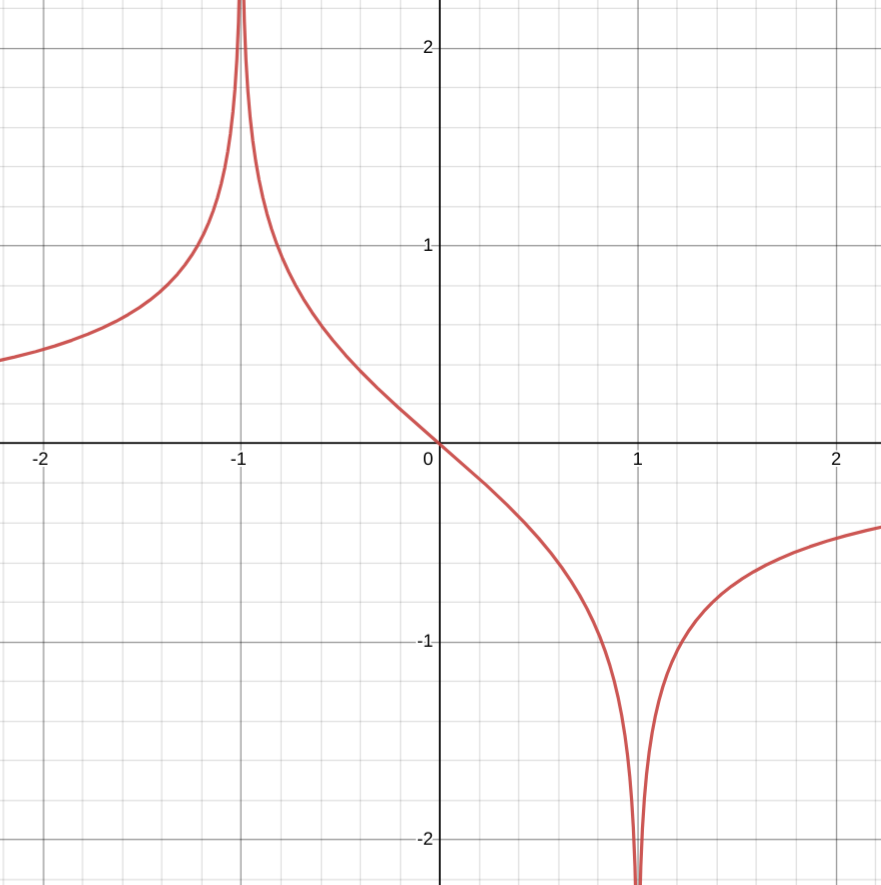
\includegraphics[width=0.3\textwidth]{fig/1.3.10.png}
    \caption{$\phi(t)$}
    \label{fig:1.3.10}
\end{figure}

\begin{itemize}
    \item $\bm{D_1=\{(t,y)|-\infty<t<-1,|y|<\infty\}}$\\
    $\phi(t)$ is not differentiable at $t=-1$ which is not included in $D_1$.
    \item $\bm{D_2=\{(t,y)|-1<t<-1,|y|<\infty\}}$\\
    $\phi(t)$ is not differentiable at $t=-1$ and $t=$ which is not included in $D_2$.
    \item $\bm{D_3=\{(t,y)|1<t<\infty,|y|<\infty\}}$\\
    $\phi(t)$ is not differentiable at $t=1$ and $t=$ which is not included in $D_3$.
\end{itemize}
\vskip1mm\hrule

\subsubsection*{Exercise 1.3.11}
According to plot of $\phi(t)$ in Fig. \ref{fig:1.3.11} we have:
\begin{figure}[h!]
    \centering
    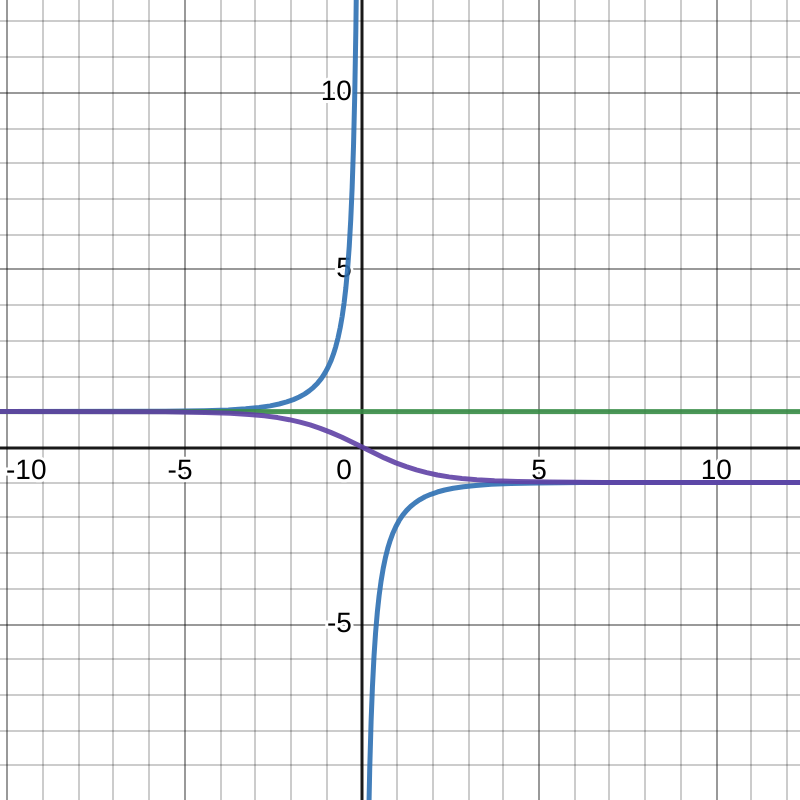
\includegraphics[width=0.3\textwidth]{fig/1.3.11.png}
    \caption{$\phi(t)=\frac{1+ce^t}{1-ce^{t}}$ for $c=-1, 0, 1$}
    \label{fig:1.3.11}
\end{figure}
\begin{enumerate}[i.]
        \item $\phi(t)$ is not differentiable at $t=-\ln{c}$ when $c>0$ and is differentiable everywhere when $c\leq0$
        \item 3 Possible regions of solution will be:
        \begin{itemize}
            \item $c>0$: $D=\{(t,y)|-\infty<t<-\ln{c},1<y<\infty\}$
            \item $c>0$: $D=\{(t,y)|-\ln{c}<t<\infty,-\infty<y<1\}$
            \item $c\leq0$: $D=\{(t,y)|-\infty<t<\infty,-1<y<1\}$
        \end{itemize}
        \item $\phi'(t)=\frac{\phi^2-1}{2}$
    \end{enumerate}
\vskip1mm\hrule

\subsubsection*{Exercise 1.3.17}

\begin{align*}
    y_1'&=+3y_1^2+3y_2^2-2y_1y_2\\
    y_2'&=-2y_1^2-2y_2^2+2y_1y_2
\end{align*}
\vskip1mm\hrule
\clearpage

\section*{1.4 Vector-Matrix Notation for Systems \xrfill[2pt]{3pt}[blue]}

\subsubsection*{Exercise 1.4.2}
To show $\forall \bm{y}\in E_n\quad ||\bm{y}||\leq|\bm{y}|\leq\sqrt{n}||\bm{y}||$
\begin{itemize}
    \item LHS Inequality
    \begin{align*}
        &\Longleftrightarrow\quad\sum_i |y_i|^2\leq(\sum_i|y_i|)^2\\
        &\Longleftrightarrow\quad\sum_i |y_i|^2\leq\sum_i|y_i|^2+\sum_{i\neq j}|y_i||y_j|\\
        &\Longleftrightarrow\qquad\qquad0\leq\sum_{i\neq j}|y_i||y_j|
    \end{align*}

    \item RHS Inequality
    \begin{align*}
        &\Longleftrightarrow\quad(\sum_i|y_i|)^2\leq n\sum_i |y_i|^2\\
        &\Longleftrightarrow\quad\sum_i|y_i|^2+\sum_{i\neq j}|y_i||y_j|\leq n\sum_i |y_i|^2\\
        &\Longleftrightarrow\quad\sum_{i\neq j}|y_i||y_j|\leq (n-1)\sum_i |y_i|^2\qquad(*)
    \end{align*}
    To prove the last inequality ($*$), we use modified AM-GM inequality, i.e., for each $y_i$ and $y_j$ we have $|y_i||y_j|\leq\frac{1}{2}(|y_i|^2+|y_j|^2)$:
    \begin{align*}
        \sum_{i\neq j}|y_i||y_j|\leq\frac{1}{2}\sum_{i\neq j}|y_i|^2+|y_j|^2=\frac{1}{2}2(n-1)\sum_i|y_i|^2
    \end{align*}
    therefore inequality ($*$) holds true.
\end{itemize}
\vskip1mm\hrule

\subsubsection*{Exercise 1.4.3}

\begin{enumerate}[(i)]
    \item 
    \begin{align*}
        &\Longleftrightarrow\quad ||\bm{y}||\geq0\\
        &\Longleftrightarrow\quad \sum_i|y_i|^2\geq0
    \end{align*}
    sum of non-negative elements is equal to zero iff all the elements equal to zero. Therefore $||\bm{y}||=0$ iff $\bm{y}=0$.
    \item 
    \begin{align*}
        &\Longleftrightarrow\quad ||c\bm{y}||=|c|||\bm{y}||\\
        &\Longleftrightarrow\quad \sum_i|cy_i|^2=|c|^2||\bm{y}||^2\\
        &\Longleftrightarrow\quad \sum_i|c|^2|y_i|^2=|c|^2||\bm{y}||^2\\
        &\Longleftrightarrow\quad |c|^2\sum_i|y_i|^2=|c|^2||\bm{y}||^2
    \end{align*}
    \item 
    \begin{align*}
        ||\bm{y}+\bm{z}||^2&=\sum_i|y_i+z_i|^2\\
        &=\sum_i(y_i+z_i)\overline{(y_i+z_i)}\\
        &=\sum_i |y_i|^2+\sum_i |z_i|^2+2\sum_i \Re\{y_i\overline{z_i}\} \\
        &\leq \sum_i |y_i|^2+\sum_i |z_i|^2+2\sum_i |y_i||z_i|\\
        &\leq \sum_i |y_i|^2+\sum_i |z_i|^2+2\sqrt{\sum_i |y_i|^2}\sqrt{\sum_i |z_i|^2}\quad (*)\\
        &=(||\bm y||+||\bm z||)^2
        \end{align*}
    where the inequality $(*)$ holds by Schwarz inequality, $|\sum_i |y_i||z_i||^2\leq\sum_i |y_i|^2\sum_i |z_i|^2$.
    % \item
    % \begin{align*}
    % &\Longleftrightarrow\quad ||\bm{y}+\bm{z}||^2\leq (||\bm{y}||+||\bm{z}||)^2\\
    %     &\Longleftrightarrow\quad ||\bm{y}+\bm{z}||^2\leq ||\bm{y}||^2+||\bm{z}||^2+2||\bm{y}||||\bm{z}||\\
    %     &\Longleftrightarrow\quad \sum_i(y_i+z_i)\overline{(y_i+z_i)}\leq ||\bm{y}||^2+||\bm{z}||^2+2||\bm{y}||||\bm{z}||\\
    %     &\Longleftrightarrow\quad \sum_i |y_i|^2+\sum_i |z_i|^2+2\sum_i y_i\overline{z_i}\leq ||\bm{y}||^2+||\bm{z}||^2+2||\bm{y}||||\bm{z}||\\
    %     &\Longleftrightarrow\quad (\sum_i y_i\overline{z_i})^2\leq ||\bm{y}||^2||\bm{z}||^2\\
    %     &\Longleftrightarrow\quad (\sum_i y_i\overline{z_i})^2\leq \sum_i |y_i|^2\sum_i |z_i|^2
    % \end{align*}
    % the last inequality is the the Cauchy-Schwarz inequality and holds true.
\end{enumerate}

\vskip1mm\hrule
\subsubsection*{Exercise 1.4.8}
Solution of first equation:
\begin{align*}
    y_1=Ce^{-t}\xrightarrow{\bm{\phi}(0)=(2,1)}y_1=2e^{-t}
\end{align*}
Then for the second equation:
\begin{align*}
    y_2''=y_1'+y_2'=-y1+y_1+y_2=y_2\rightarrow y_2=C_1e^{-t}+C_2e^{t}
\end{align*}
Using $\bm{\phi}(0)=(2,1)$:
\begin{align*}
    C_1+C_2&=1\\
    -C_1+C_2&=3
\end{align*}
therefore $y_2=-1e^{-t}+2e^{t}$.\\
And the valid interval of $t$ is $I=(-\infty,+\infty)$.
\vskip1mm\hrule

\subsubsection*{Exercise 1.4.11}
Let $v:=y_1+y_2$:
\begin{align*}
    v'=2v+f(t)
\end{align*}
then the homogeneous solution will be:
\begin{align*}
    v=Ce^{2t}\xrightarrow{\bm{\phi}(0)=(0,0)}v=0 \rightarrow y_1=-y_2
\end{align*}
\vskip1mm\hrule
\clearpage

\section*{1.6 Existence, Uniqueness and Continuity \xrfill[2pt]{3pt}[blue]}

\subsubsection*{Exercise 1.6.5}
For a collections of points to construct a region (open subset), we must have for each point in the subset a ball of radius $\epsilon>0$ centered on that point, in the region.
\begin{enumerate}[(a)]
    \item Is a region.
    \item Is NOT a region. Points on the boundary cannot have a neighborhood.
    \item IS a region.
    \item IS a region.
\end{enumerate}
\vskip1mm\hrule


\subsubsection*{Exercise 1.6.8}
\begin{enumerate}[(a)]
    \item 
    \begin{enumerate}[(i)]
        \item $\phi(t)$ is differentiable over $t\in(-\infty, 0)$
        \item $(t,\phi(t))\in D$ for each $t\in(-\infty,0)$, where $D=\{(t,y)| -\infty<t<0, y>0\}$
        \item $\phi'(t)=\phi^2(t)$
    \end{enumerate}
    \item For the defined $D$ in part (a), both $f=y^2$ and $f'=2y$ are continuous. Given the initial value $(-1, 1)$ the solution of $\phi(t)=-1/t$ is unique.
    \item As mentioned in part (a), the largest interval for $t$ is $(-\infty, 0)$.
\end{enumerate}
\vskip1mm\hrule

\subsubsection*{Exercise 1.6.10}
Since $\bm{f}$ and $\partial\bm{f}/\partial y_k$ are continuous, then for a given initial value in the defined region of $D$, then a unique solution $\bm\phi$ exists.
\vskip1mm\hrule

\subsubsection*{Exercise 1.6.16}
\begin{enumerate}[(a)]
    \item 
    $\phi(t)$ is not a solution since at $t=0$ it is not differentiable.
    \item Yes, it is continuous.
    \item No, it is not continuous at $t=0$.
    \item ?
\end{enumerate}
\vskip1mm\hrule
\clearpage

\section*{1.7 The Gronwall Inequality \xrfill[2pt]{3pt}[blue]}

\subsubsection*{Exercise 1.7.2}
Let $K=0$ and $g(t)=1 \quad\forall t\in[0,1]$ in Gronwall inequality, then:
\begin{align*}
    f(t)\leq0\exp(\int_0^t1ds)=0
\end{align*}
The only continuous function on $t\in[0,1]$ satisfying $f(t)\leq\int_0^tf(s)ds$ is $f(t)=0\quad\forall t\in[0,1]$.
\vskip1mm\hrule

\subsubsection*{Exercise 1.7.3}
Let $U(t)=K_1+\epsilon(t-\alpha)+K_2\int_{\alpha}^{t}f(s)ds=K_1+K_2\int_{\alpha}^{t}(\frac{\epsilon}{K_2}+f(s))ds$, then we have $f(t)\leq U(t)$ and $U(\alpha)=K_1$:
\begin{align*}
    U'(t)=\epsilon+K_2f(t)=K_2(f(t)+\frac{\epsilon}{K_2})&\leq K_2(U(t)+\frac{\epsilon}{K_2})\\
    U'(t)-K_2(U(t)+\frac{\epsilon}{K_2})&\leq0\\
    U'(t)\exp(-K_2(t-\alpha))-K_2(U(t)+\frac{\epsilon}{K_2})\exp(-K_2(t-\alpha))&\leq0\\
    [(U(t)+\frac{\epsilon}{K_2})\exp(-K_2(t-\alpha))]'&\leq0\\
    (U(t)+\frac{\epsilon}{K_2})\exp(-K_2(t-\alpha))-U(\alpha)-\frac{\epsilon}{K_2}&\leq0\\
    (U(t)+\frac{\epsilon}{K_2})\exp(-K_2(t-\alpha))-K_1-\frac{\epsilon}{K_2}&\leq0\\
    U(t)\leq-\frac{\epsilon}{K_2}+K_1\exp(K_2(t-\alpha))+&\frac{\epsilon}{K_2}\exp(K_2(t-\alpha))\\
    U(t)\leq K_1\exp(K_2(t-\alpha))+&\frac{\epsilon}{K_2}(\exp(K_2(t-\alpha))-1)
\end{align*}
since $f(t)\leq U(t) \quad\forall t\in[\alpha, \beta]$:
\begin{align*}
    f(t)\leq K_1\exp(K_2(t-\alpha))+\frac{\epsilon}{K_2}(\exp(K_2(t-\alpha))-1)
\end{align*}
\vskip1mm\hrule
\clearpage

\section*{2.3 Linear Homogeneous Systems \xrfill[2pt]{3pt}[blue]}

\subsubsection*{Exercise 2.3.6}
Suppose they are linearly dependent, then there exists $a_1, a_2, a_3\in \mathbb{E}$ not all zero such that:
\begin{align*}
    a_1v_1+a_2v_2+a_3v_3=0\\
    \left( \begin{array}{c} a_1 \\ a_2+a_3 \\ a_3 \end{array} \right)=\left( \begin{array}{c} 0 \\ 0 \\ 0 \end{array} \right) 
\end{align*}
then $a_1=a_3=a_2=0$ which is a contradiction and $v_1, v_2, v_3$ are linearly independent.
\vskip1mm\hrule

\subsubsection*{Exercise 2.3.8}
Suppose they are linearly dependent, then there exists $a_1, a_2\in \mathbb{E}$ not all zero such that:
\begin{align*}
    a_1e^{r_1t}+a_2e^{r_2t}=0 \quad (\forall t\in\R)
\end{align*}
since $r_1\neq r_2$, then both $a_1=a_2=0$ which is contradiction and $v_1, v_2$ are linearly independent.
\vskip1mm\hrule

\subsubsection*{Exercise 2.3.23}
First we show that $\bm\Phi$ is a solution matrix:
\begin{itemize}
    \item
    \begin{align*}
        \left( \begin{array}{c} -\sin t \\ -\cos t  \end{array}\right)=
        \left( \begin{array}{cc} 0 & 1 \\ -1 & 0  \end{array}\right)
        \left( \begin{array}{c} \cos t \\ -\sin t  \end{array}\right)
    \end{align*}
    \item 
    \begin{align*}
        \left( \begin{array}{c} \cos t \\ -\sin t  \end{array}\right)=
        \left( \begin{array}{cc} 0 & 1 \\ -1 & 0  \end{array}\right)
        \left( \begin{array}{c} \sin t \\ \cos t  \end{array}\right)
    \end{align*}
\end{itemize}
now that $\bm\Phi$ is a solution matrix, if $\det\bm\Phi\neq0\quad\forall t\in I$, then $\bm\Phi$ is a fundamental matrix. Since $\det\bm\Phi=1\quad\forall t\in I$ then $\bm\Phi$ is a fundamental matrix.
\vskip1mm\hrule

\subsubsection*{Exercise 2.3.24}
First we show that $\bm\Phi$ is a solution matrix:
\begin{itemize}
    \item
    \begin{align*}
        \left( \begin{array}{c} r_1\exp(r_1t) \\ r_1^2\exp(r_1t)  \end{array}\right)=
        \left( \begin{array}{cc} 0 & 1 \\ -a_2 & -a_1 \end{array}\right)
        \left( \begin{array}{c} \exp(r_1t)  \\ r_1\exp(r_1t)   \end{array}\right)
    \end{align*}
    \item 
    \begin{align*}
        \left( \begin{array}{c} r_2\exp(r_2t) \\ r_2^2\exp(r_2t)  \end{array}\right)=
        \left( \begin{array}{cc} 0 & 1 \\ -a_2 & -a_1 \end{array}\right)
        \left( \begin{array}{c} \exp(r_2t)  \\ r_2\exp(r_2t)   \end{array}\right)
    \end{align*}
\end{itemize}
the equation above holds since $r_1, r_2$ are solutions of $z^2+a_1z+a_2=0$.
Now that $\bm\Phi$ is a solution matrix, if $\det\bm\Phi\neq0\quad\forall t\in I$, then $\bm\Phi$ is a fundamental matrix.\\
Using Abel's Formula, since $\det\bm\Phi(0)=r_2-r_1\neq 0$ then $\det\bm\Phi\neq0\quad\forall t\in I$ and therefore $\bm\Phi$ is a fundamental matrix.
\vskip1mm\hrule

\subsubsection*{Exercise 2.3.27}
\begin{enumerate}[(a)]
    \item First we show that $\bm\Phi$ is a solution matrix:
    \begin{itemize}
        \item
        \begin{align*}
            \left( \begin{array}{c} 2t \\ 2  \end{array}\right)=
            \left( \begin{array}{cc} 0 & 1 \\ -2/t^2 & 2/t \end{array}\right)
            \left( \begin{array}{c} t^2  \\ 2t   \end{array}\right)
        \end{align*}
        \item 
        \begin{align*}
            \left( \begin{array}{c} 1 \\ 0  \end{array}\right)=
            \left( \begin{array}{cc}0 & 1 \\ -2/t^2 & 2/t \end{array}\right)
            \left( \begin{array}{c} t  \\ 1   \end{array}\right)
        \end{align*}
    \end{itemize}
    Now that $\bm\Phi$ is a solution matrix, if $\det\bm\Phi\neq0\quad\forall t\in I$, then $\bm\Phi$ is a fundamental matrix.\\
Using Abel's Formula, since $\det\bm\Phi(1)=2\neq 0$ then $\det\bm\Phi\neq0\quad\forall t\in I$ and therefore $\bm\Phi$ is a fundamental matrix.
    \item No, since the interval $I$ on which solution $\Phi$ is defined, does not include zero.
\end{enumerate}
\vskip1mm\hrule

\subsubsection*{Exercise 2.3.28}
Since we can write
\begin{align*}
    \left( \begin{array}{cc} \cos t & \sin t \\ -\sin t & \cos t \end{array}\right)=
    \left( \begin{array}{cc} e^{it} & e^{-it} \\ ie^{it} & -ie^{-it} \end{array}\right)
    \left( \begin{array}{cc} 0.5 & -0.5i \\ 0.5 & 0.5i \end{array}\right)
\end{align*}
then it is also a fundamental matrix.\\
Another real fundamental matrix:
\begin{align*}
    \left( \begin{array}{cc} \cos t & \sin t \\ -\sin t & \cos t \end{array}\right)
    \left( \begin{array}{cc} 1 & 0 \\ 1 & 1 \end{array}\right)=
    \left( \begin{array}{cc} \cos t & \sin t \\ -\sin t + \cos t & \cos t \end{array}\right)
\end{align*}
\vskip1mm\hrule
\clearpage


\section*{2.4 Linear Nonhomogeneous Systems \xrfill[2pt]{3pt}[blue]}

\subsubsection*{Exercise 2.4.5}
From \textbf{Exercise 2.3.27} we know a fundamental matrix of the homogeneous equation on $I=\R\setminus\{0\}$:
\begin{align*}
    \bm\Phi(t)=
    \left( \begin{array}{cc} t^2 & t \\ 2t & 1 \end{array}\right)
\end{align*}
where its inverse will be:
\begin{align*}
    \bm\Phi^{-1}(t)=\frac{-1}{t^2}
    \left( \begin{array}{cc} 1 & -t \\ -2t & t^2 \end{array}\right)
\end{align*}
The particular solution $\psi(t)$ with initial conditions of $\psi(2)=\left( \begin{array}{c} 0 \\ 0\end{array}\right)$ will be calculated using Variation of Constants formula:
\begin{align*}
    \psi(t)&=\bm\Phi(t)\int_2^t \bm\Phi^{-1}(s)g(s)ds\\
    &=\bm\Phi(t)\int_2^t \left( \begin{array}{cc} -1 & s \\ 2s & -s^2 \end{array}\right)\left( \begin{array}{c} s^2 \\ s\end{array}\right)ds\\
    &=\bm\Phi(t)\int_2^t \left( \begin{array}{c} 0 \\ s^3\end{array}\right)ds\\
    &=\bm\Phi(t)\left( \begin{array}{c} 0 \\ t^4/4-4\end{array}\right)\\
    &=\left( \begin{array}{c} t^5/4-4t \\ t^4/4-4\end{array}\right)
\end{align*}
Now we find the homogeneous solution $\phi_h(t)$ using the intial condition of $\phi_h(2)=\left( \begin{array}{c} 1 \\ 4\end{array}\right)=\bm\Phi(2)\bm c$:
\begin{align*}
    \bm{c}=\bm\Phi^{-1}(2)\left( \begin{array}{c} 1 \\ 4\end{array}\right)=\frac{-1}{4}\left( \begin{array}{c} -7 \\ 12\end{array}\right)
\end{align*}
therefore
\begin{align*}
    \phi_h(t)=\frac{-1}{4}\left( \begin{array}{c} 7t^2+12t \\ -14t+12\end{array}\right)
\end{align*}
hence the general solution will be $\phi(t)=\phi_h(t)+\psi(t)$.
\vskip1mm\hrule

\subsubsection*{Exercise 2.4.6}
\begin{enumerate}[(a)]
    \item Let $y_1=y$ and $y_2=y'$ then:
    \begin{align*}
        y_1'&=y_2\\
        y_2'&=-q(t)y_1-p(t)y_2+f(t)
    \end{align*}
    then $\left( \begin{array}{c} \phi_1 \\ \phi_1'\end{array}\right)$ and $\left( \begin{array}{c} \phi_2 \\ \phi_2'\end{array}\right)$ are the solutions of this system of differential equations. Since $\phi_1$ and $\phi_2$ are linearly independent (? not sure about vectors!), then the matrix $\bm\Phi(t)=\left( \begin{array}{cc} \phi_1 & \phi_2 \\ \phi_1' & \phi_2'\end{array}\right)$ is a fundamental matrix.

    \item 
    By having $g(t)=\left( \begin{array}{c} 0 \\ f(t)\end{array}\right)$, using Variation of Constants formula:
    \begin{align*}
        \psi(t)&=\bm\Phi(t)\int_2^t \bm\Phi^{-1}(s)g(s)ds\\
        &=\bm\Phi(t)\int_2^t \frac{1}{\det\bm\Phi}\left( \begin{array}{cc} \phi_2' & -\phi_2 \\ -\phi_1' & \phi_1 \end{array}\right)\left( \begin{array}{c} 0 \\ f(s)\end{array}\right)ds
    \end{align*}
    
    \item
    \begin{align*}
        \left( \begin{array}{c} \psi_1(t) \\ \psi_2(t)\end{array}\right)&=\bm\Phi(t)\int_2^t \bm\Phi^{-1}(s)g(s)ds\\
        &=\bm\Phi(t)\int_2^t \frac{f(s)}{\phi_1\phi_2'-\phi_2\phi_1'}\left( \begin{array}{c} -\phi_2 \\ \phi_1\end{array}\right)ds
    \end{align*}
    and we know that $\psi_1'=\psi_2$ by definition of the ODE system.
\end{enumerate}

\vskip1mm\hrule
\clearpage


\section*{2.5 Linear Systems with Constant Coefficients \xrfill[2pt]{3pt}[blue]}

\subsubsection*{Exercise 2.5.3}
\begin{align*}
    \exp{M}.\exp{P}=&(I+\frac{M}{1!}+\frac{M^2}{2!}+\dots)(I+\frac{P}{1!}+\frac{P^2}{2!}+\dots)\\
    &=I+(P+M)+\frac{M^2+P^2+2MP}{2!}+\frac{M^3+P^3+3MP^2+3PM^2}{3!}+\dots\\
    &=\exp{(M+P)}
\end{align*}
last equality holds since $M$ and $P$ are commutative.
\vskip1mm\hrule

\subsubsection*{Exercise 2.5.5}
The power series of $\exp{tA}$ is convergent for $t\in(-\infty,+\infty)$, so its integration/differentiation is allowed. We use the same differentiation rule of power series for the matrix power series, therefore:
\begin{align*}
    (\exp{tA})'&=A+\frac{tA^2}{1!}+\frac{t^2A^3}{2!}+\dots\\
    &=A(I+\frac{tA}{1!}+\frac{t^2A^2}{2!}+\dots)\\
    &=A\exp{tA}
\end{align*}
\vskip1mm\hrule

\subsubsection*{Exercise 2.5.6}
The exponents are commutable: $(tA)(-tA)=(-tA)(tA)$.
\\
Since $(\exp{tA})(\exp{-tA})=(\exp{-tA})(\exp{tA})=\exp(tA-tA)=\exp(0A)=I$, $\exp{-tA}$ is the inverse of $\exp{tA}$.
\vskip1mm\hrule
\clearpage

\end{document}

